% Submission version (peer-blind). Target journal: Rapid Prototyping Journal (Emerald).
% Author identity intentionally omitted for double-anonymous review.
% RPJ house style reflected below (SFTF_style_template.dotx): A4, 12pt double-spaced
% review copy, Emerald structured abstract, keywords + article classification,
% Roman-numeral tables, Harvard (author-date) citations, running short-title header.
% RPJ length policy: <= 9,000 words including abstract, references, and all text in
% tables/figures/appendices (each float counted as ~280 words).
\documentclass[12pt,a4paper]{article}
\usepackage[T1]{fontenc}
\usepackage[utf8]{inputenc}
\usepackage[margin=25mm]{geometry}
\usepackage{amsmath,amssymb,bm}
\usepackage{booktabs}
\usepackage{graphicx}
\usepackage{float}
\usepackage[labelfont=bf,labelsep=period]{caption}
\usepackage[authoryear,round]{natbib}
\usepackage{setspace}
\usepackage{fancyhdr}
\usepackage[hidelinks]{hyperref}
\setlength{\emergencystretch}{1em}
\setlength{\headheight}{14pt}
\doublespacing

% Emerald / RPJ house style: Roman-numeral tables and Harvard author-date citations.
\renewcommand{\thetable}{\Roman{table}}

% Peer-blind running header (short title only; no author identity).
\pagestyle{fancy}\fancyhf{}
\fancyhead[R]{\small Does a Local Metric Help Anisotropic Alpha Reconstruction?}
\fancyfoot[C]{\thepage}
\renewcommand{\headrulewidth}{0.4pt}

\title{Does a Local Metric Help Anisotropic Alpha-Complex Surface
Reconstruction for Additive Manufacturing? A Frozen Held-Out Evaluation}
\author{}
\date{}

\begin{document}
\maketitle
\thispagestyle{fancy}

\begin{abstract}
\noindent\textbf{Purpose.} In additive-manufacturing (AM) reverse-engineering and
scan-to-print workflows a surface mesh is reconstructed from a scanned point cloud,
and scale selection for alpha-complex reconstruction governs printed-part fidelity.
This paper asks whether a local symmetric-positive-definite (SPD) metric derived from
a directed relation-tensor field adds value beyond established density-adaptive and
normal-anisotropic alpha baselines.

\noindent\textbf{Design/methodology/approach.} A predeclared, frozen held-out
protocol with strict information boundaries evaluates the methods on a synthetic
six-family panel and a real-mesh corpus, scoring every candidate against a strict
casewise per-endpoint baseline envelope on geometry and topology.

\noindent\textbf{Findings.} The primary result is negative: on real held-out meshes
the normal-anisotropic baseline attains the best mean surface F-score ($0.868$) and
no local-metric variant exceeds it (the closest trails by $0.094$, bootstrap 95\% CI
$[-0.11,-0.08]$, clearing the envelope in 2 of 40 cases). A weighted (regular/power)
alpha complex that changes connectivity strictly improves the density baseline on
both synthetic and real data, and a deployed fail-closed exact-construction fallback
never certifies an unvalidated result.

\noindent\textbf{Practical implications.} For AM reconstruction quality assurance a
well-regularised normal-based metric remains the strong default; a heavier local
metric is not worth its cost, whereas the weighted-alpha connectivity change and the
fail-closed fallback are safe, reusable upgrades.

\noindent\textbf{Originality/value.} A rigorous, reproducible held-out comparison
that quantifies the (non-)value of a local-metric anisotropic alpha for AM
reconstruction, together with a better density baseline, a safety fallback, and a
documented universal failure of removal-based false-bridge interventions.
\end{abstract}

\vspace{0.5em}
\noindent\textbf{Keywords.} Surface reconstruction; Alpha complex; Additive
manufacturing; Reverse engineering; Anisotropic metric; Held-out evaluation

\vspace{0.25em}
\noindent\textbf{Article classification.} Research paper

\section{Introduction}
Reverse-engineering and scan-to-print pipelines in additive manufacturing (AM) begin
by reconstructing a surface mesh from a scanned point cloud, and the geometric
fidelity and topological soundness of that reconstruction propagate directly into the
printed part. A boundary that is over-filled fuses features that should be separate;
a boundary that is under-filled opens holes that break watertightness and make the
model unslicealable without repair. Because the downstream slicer assumes a clean,
orientable, watertight shell, reconstruction error is not cosmetic: it determines
whether a scanned part can be re-manufactured at all, and how much manual repair the
operator must perform before printing. Reconstruction quality is therefore a genuine
AM concern, not only a computational-geometry one.

The alpha complex \citep{edelsbrunner1994} is a classical and still widely used tool
for this task: from a fixed Delaunay triangulation of the input points it selects a
subcomplex governed by a scale parameter $\alpha$, interpolating between the point set
(small $\alpha$) and the convex hull (large $\alpha$). Its appeal is that it is
parameter-light, provably a subcomplex of the Delaunay triangulation, and comes with a
clean topological interpretation. Its weakness is equally well known: a single global
scale cannot simultaneously avoid over-fill in dense regions and topology loss in
sparse regions when the sampling density varies in space, as it always does for real
scans of parts with mixed feature sizes.

Two families of remedy are established. The first is \emph{density-adaptive} alpha,
which normalises each tetrahedron's circumradius by the local $k$-nearest-neighbour
(kNN) spacing so that the effective scale tracks the sampling density (we denote this
baseline B4). The second is \emph{normal-anisotropic} alpha, which replaces the
isotropic Euclidean radius with a regularised local principal-component (PCA) SPD
metric carrying a planarity-weighted penalty along the estimated surface normal, so
that the complex prefers to grow tangentially along the surface rather than across it
(B5). Both are strong, cheap, and require only local neighbourhood computations.

Against this backdrop a richer construction has been proposed. From directed kNN
scale contrast and receiver-direction imbalance one can build a \emph{signed,
trace-free relation tensor} field, map it through bounded log-eigenvalues to a local
SPD metric, and score the alpha complex under that metric (we call this candidate P1).
A confidence-gated conservative variant falls back to the density baseline on cells
where the field is deemed unreliable (P2). Such a field encodes more of the local
directional structure than a symmetric normal tensor can, and it is natural to hope
that this extra structure sharpens reconstruction where normals alone are ambiguous.
Whether that hope survives contact with realistic data is exactly the question a
practitioner deciding what to deploy must answer.

\paragraph{Question.} Does the added complexity of a local SPD metric provide
reconstruction value beyond the existing density (B4) and normal-anisotropic (B5)
baselines, under an evaluation strict enough to be trusted?

\paragraph{Contributions.} (1) A predeclared frozen held-out protocol with strict
information boundaries, applied to a synthetic six-family panel and to a real-mesh
corpus, that scores every candidate against a casewise per-endpoint baseline
\emph{envelope} rather than a mean. (2) A quantitative, \emph{negative} answer: the
local SPD metric does not beat the normal-anisotropic baseline on real held-out data,
and a small mean gain on the synthetic panel does not survive the envelope test.
(3) A weighted regular (power) alpha complex, M1, that changes the connectivity itself
and strictly improves the density baseline on both synthetic and real data. (4) A
deployed fail-closed exact-construction fallback with a no-silent-false-safe
guarantee, and a comprehensive negative map showing that removal-based false-bridge
interventions fail universally, with an explanation of why.

We stress at the outset that this is an honest negative/limits study. We do not claim
to beat prior art; we claim to have measured, carefully, that a specific and
intuitively appealing addition does not help, and to have isolated the two pieces that
do.

\section{Related work}
\subsection{Alpha shapes and their weighted generalisation}
Alpha shapes and the three-dimensional alpha complex \citep{edelsbrunner1994} select a
subcomplex of the Delaunay triangulation by a single scale, and remain a default
reconstruction primitive because of their simplicity and topological guarantees. The
weighted (regular, or power) generalisation \citep{edelsbrunner1992} assigns each site
a scalar weight and replaces the Delaunay triangulation by the regular triangulation of
the weighted points, obtained as a lower convex hull of a lift into one higher
dimension. Weights let sites of different importance or density occupy different
effective radii; crucially, they change the underlying \emph{connectivity}, not merely
the order in which a fixed set of simplices is admitted. Our M1 candidate is a
density-driven instance of this classical device, and its ability to remove simplices
that a fixed Delaunay triangulation would force to remain is the reason it can do what
rescoring a fixed complex cannot.

\subsection{Density-adaptive and anisotropic reconstruction}
Normalising the alpha scale by local sampling density is a standard way to handle
non-uniform clouds and underlies our B4 baseline. Anisotropic reconstruction, in
which the notion of ``nearby'' is stretched by a local metric rather than a scalar
radius, is likewise well established; the most common construction estimates a local
tangent frame by principal-component analysis and penalises growth along the normal,
which presupposes consistently oriented normals \citep{hoppe1992}. Our B5 baseline is
a regularised, planarity-weighted member of this family. The relation-tensor metric
(P1/P2) evaluated here is a more elaborate anisotropy that additionally encodes
directed scale contrast; the empirical question is whether that elaboration buys
anything over the PCA metric.

\subsection{Automatic scale selection}
Because a single global $\alpha$ is inadequate, a body of work selects the scale
automatically, for example by persistence of topological features across the
filtration or by resampling stability of the reconstructed surface. Our B3 baseline
instantiates this idea as an unlabelled persistence-plus-resampling-stability selector,
and we further probe a resampling-persistence gate as a possible false-bridge detector.
As reported below, that gate does not discriminate true from false bridges on our data
(discrimination near chance), which is itself informative about the limits of local
stability signals.

\subsection{Watertight labelling of Delaunay tetrahedra}
A distinct and powerful family reconstructs a watertight surface by labelling each
Delaunay tetrahedron as inside or outside, typically via a global minimum-cut on the
tetrahedral adjacency graph with visibility or normal-consistency terms
\citep{labatut2009}. This global labelling can, in principle, resolve exactly the
thin-gap configurations that defeat every local method we test. We do not implement it
here---it is a separate, large engineering effort---but we identify it as the one
untested avenue that our negative results do not foreclose, and we discuss why it is
the natural next step rather than yet another local metric.

\subsection{Evaluation methodology}
Reconstruction papers frequently report improvements as gains in a mean score over a
convenience set of shapes, tuned and evaluated on overlapping data. We deliberately
adopt a stricter stance: a predeclared protocol, frozen scales, strict information
boundaries between calibration and evaluation, and a casewise per-endpoint baseline
envelope that a candidate must clear \emph{case by case} rather than on average. This
methodology is a contribution in its own right, because it is precisely what converts
an appealing mean gain (which P2 exhibits on one synthetic profile) into a verdict of
no value.

\section{Methods}
\subsection{Problem set-up and evaluation endpoints}
Given an observed point cloud sampled from an unknown surface, a reconstruction method
returns a triangulated surface. We evaluate each reconstruction against a dense
reference on complementary endpoints so that a method cannot trade topology for
geometry unnoticed. The \emph{surface F-score} is the harmonic mean of precision and
recall of reconstructed versus reference surface samples under a fixed distance
tolerance (higher is better) and is our headline geometric-completeness measure. The
\emph{geometric loss} is a normalised two-sided (Chamfer-type) surface distance
between reconstruction and reference (lower is better). Topological soundness is
summarised by the \emph{Betti error}, the absolute discrepancy in Betti numbers
against the ground-truth shell, and by the count of \emph{nonmanifold edges} (edges
incident to other than two triangles), both of which a printable shell should drive to
zero. Finally, we count \emph{false-bridge edges}: edges that connect points belonging
to distinct ground-truth surface sheets, i.e.\ spurious connectivity that fuses
features which should stay separate. A method is credible only if it improves the
F-score without regressing topology, which is why our acceptance test is casewise and
multi-endpoint rather than a single averaged number.

\subsection{Baselines and candidates}
B0--B3 are, respectively, a convex hull; a fixed normalised-radius alpha; an
exhaustive critical-scale oracle allowed to consult the dense reference (an upper
bound, not a deployable method); and an unlabelled persistence-plus-resampling-
stability scale selector. B4 divides each tetrahedron's Euclidean circumradius by the
geometric-mean kNN spacing of its vertices, giving density adaptation. B5 combines a
regularised local PCA SPD metric with the same density normalisation and a
planarity-weighted normal penalty, giving normal anisotropy. P1 forms the
relation-tensor SPD metric described next; P2 adds a $\max(\mathrm{P1},\mathrm{B4})$
guard on low-confidence cells so that it can never score below the density baseline.

Critically, B4, B5, P1 and P2 all select subcomplexes of \emph{one fixed isotropic
Delaunay triangulation} by a per-cell scalar threshold. They differ only in how they
score a cell, never in which cells exist. It follows that a false-bridge tetrahedron
already present in that triangulation cannot be removed by any of them without also
removing legitimate incident simplices---a structural ceiling that motivates M1.

\subsection{The relation-tensor local metric (P1/P2)}
For each site the field construction compares directed kNN scale contrast against its
neighbours and measures the imbalance of receiver directions, yielding a signed,
trace-free relation tensor $\bm{T}$ at that site. The antisymmetric and deviatoric
structure of $\bm{T}$ encodes directional relationships that a symmetric normal tensor
cannot represent. To obtain a usable metric, $\bm{T}$ is symmetrised and passed through
bounded log-eigenvalues, $\bm{M}=\exp\!\big(\mathrm{clip}(\log\text{-spectrum})\big)$,
which guarantees a well-conditioned SPD metric with eigenvalues confined to a fixed
band, preventing degenerate stretches. Cells are then scored by their circumradius
measured under $\bm{M}$ instead of the Euclidean radius. P2 additionally computes a
per-cell confidence from the field and, where confidence is low, falls back to the B4
score, so P2 is by construction a conservative interpolation between P1 and the density
baseline.

\subsection{M1: weighted regular (power) alpha complex}
M1 departs from the fixed-triangulation family by changing the connectivity itself.
Each point receives a density weight $w_i=(s\cdot\mathrm{spacing}_i)^2$, where
$\mathrm{spacing}_i$ is its local kNN spacing and $s\ge 0$ is a single global weight
scale. The regular (weighted) triangulation is the lower convex hull of the lift
\begin{equation}
p_i\;\longmapsto\;\big(p_i,\;\lVert p_i\rVert^2-w_i\big),
\label{eq:lift}
\end{equation}
so that with $w\equiv 0$ the construction reproduces the ordinary Delaunay
triangulation and M1 strictly generalises B4. Cells are scored by the \emph{proper}
weighted (power) circumradius normalised by kNN spacing. This detail is not cosmetic:
scoring the weighted connectivity with the \emph{ordinary} circumradius reintroduces
nonmanifold edges and Betti regressions, whereas the power circumradius---the natural
radius in the weighted setting---removes them, so the two design choices (weighted
connectivity, power scoring) must be made together. Because a sufficiently large weight
submerges a point beneath the lower hull and deletes it from the triangulation, the
weight scale $s$ is capped; we freeze $s$ on calibration data.

\subsection{G4: deployed fail-closed exact fallback}
Floating-point Delaunay construction can, on adversarial inputs, produce a topologically
invalid complex. For a deployment that must never silently certify a bad result, we
attach an exact Euclidean Delaunay backend that runs under host validation and, on
acceptance, injects its validated connectivity into the actual selection path. On any
refusal---a point-count cap exceeded, an exact cospherical ambiguity, host rejection,
or backend timeout or malformed output---the method \emph{fails closed} to a floating
construction that is explicitly labelled non-exact, and records the specific reason.
The \emph{certified} outcome is reachable only after full validation passes; every
failure mode records a reason and is never silently treated as safe. A suite of nine
failure-mode tests exercises each refusal path, and the default 96-point evaluation
panel always fails closed under the deliberately conservative 64-point cap. The
guarantee is deliberately narrow: G4 certifies only the base Delaunay connectivity, not
the anisotropic complex built on top of it.

\subsection{Frozen held-out protocol and information boundaries}
Every method's scale, and M1's weight scale $s$, is frozen on a \emph{calibration} set;
no tuning of any kind is permitted on the held-out set. Reference clouds and
ground-truth labels enter calibration and final scoring only---never held-out
selection---so that no method can peek at the answer while choosing its complex. Each
candidate is judged against the strict casewise per-endpoint baseline \emph{envelope}
$\max(\mathrm{B4},\mathrm{B5})$: to clear the gate on a case it must match or beat,
endpoint by endpoint, whichever baseline is stronger \emph{on that case}. This is a far
harder bar than beating either baseline on average, and it is what prevents a candidate
from claiming victory by winning easy cases while losing hard ones.

\section{Experiments}
\subsection{Synthetic six-family panel}
The synthetic panel comprises six shape families chosen to exercise distinct failure
modes---disconnected parts, closely opposing sheets, thin tubes, and mixed-density
regions among them. Scales are frozen on a calibration instance of the six families,
and evaluation runs four held-out profiles (a base profile plus sparser, noisier, and
harder-geometry variants) over three paired random seeds, so that every method sees
identical clouds. The panel is intentionally adversarial and, as we show, contains one
pathology (an inter-sheet gap smaller than the sample spacing) that no local method can
resolve.

\subsection{Real-mesh corpus and splits}
The real corpus draws watertight meshes from a public 3D-printing model set
\citep{zhou2016thingi10k} together with CAD primitives. Observed clouds are
area-weighted surface samples with additive noise, and dense reference clouds are drawn
from the same meshes. Scales are frozen on a calibration mesh set and evaluated on a
disjoint held-out mesh set across density and noise splits, for 40 held-out cases in
total. This is the setting that matters for the AM question, because it is where the
baselines' assumptions (well-defined normals on smooth shells) actually hold.

\section{Results}
\subsection{Synthetic preflight}
The frozen confidence-fallback variant P2 preserves the density guard (zero violations)
but fails the strict casewise envelope on all four held-out profiles, with mean
F-score margins $-0.048$, $+0.0002$, $-0.049$ and $-0.049$. The one near-zero, slightly
positive mean margin is instructive: it is exactly the kind of small averaged gain that
a weaker evaluation would report as an improvement, yet under the casewise envelope it
is not evidence of value. On calibration, M1 at weight scale $s=0.375$ strictly
dominates B4 on every endpoint (Table~\ref{tab:syn})---higher F-score, lower geometric
loss, no Betti or nonmanifold regression, and fewer false-bridge edges---whereas the
normal-anisotropic baseline B5 is topologically degenerate on this panel (Betti error
$105$, $175$ nonmanifold edges), an artefact of the panel's thin-gap pathology rather
than a property of B5 in general. On the held-out envelope M1 is $4$--$5\times$ closer
than the previous best (per-profile F-margins
$-0.0105/{-}0.0005/{-}0.0003/{-}0.0109$) but does not clear it; the residual gap is
dominated by one family's false bridges, which we dissect below.

\begin{table}[t]\centering
\caption{Synthetic calibration, frozen multipliers. M1 ($s{=}0.375$) strictly
dominates the density baseline B4 on every endpoint. B5's topology figures reflect a
panel-specific thin-gap pathology, not its behaviour on real meshes.}
\label{tab:syn}
\begin{tabular}{lccccc}
\toprule
Method & F-score & Geom.\ loss & Betti err. & Bridge edges & Nonmanifold \\
\midrule
B4              & 0.365 & 0.1802 & 9   & 48 & 0 \\
M1 ($s{=}0.375$) & \textbf{0.384} & \textbf{0.1730} & 9 & \textbf{46} & 0 \\
B5              & 0.391 & 0.1824 & 105 & 61 & 175 \\
\bottomrule
\end{tabular}
\end{table}

\subsection{Real held-out data (the headline)}
Table~\ref{tab:real} is the central result. On real meshes the normal-anisotropic
baseline B5 is clearly the strongest (mean F-score $0.868$, mean geometric loss
$0.058$), and no local-metric candidate exceeds it. The closest candidate, M1, trails
by $0.094$ with a bootstrap 95\% confidence interval that excludes zero, and clears the
casewise envelope in only 2 of 40 cases; the relation-tensor candidates P1 and P2 trail
by $0.14$ and clear it in 0 of 40. Figure~\ref{fig:fscore} shows the ranking and
Figure~\ref{fig:margin} the candidate margins against the baseline envelope with 95\%
confidence intervals; every candidate interval lies entirely below zero. This reverses
the synthetic picture: on smooth real meshes the well-defined normals make B5 excel,
while its synthetic degeneracy was an artefact of a panel pathology rather than a real
weakness. The practical reading is direct---the local SPD metric adds no value on real
data, and the honest default remains a well-regularised normal-based metric.

M1 nonetheless keeps its secondary win: it beats the density baseline B4 on real data
too ($0.774$ vs.\ $0.728$), confirming that the connectivity change transfers from
synthetic to real, even though it does not close the gap to B5.

\begin{figure}[t]\centering
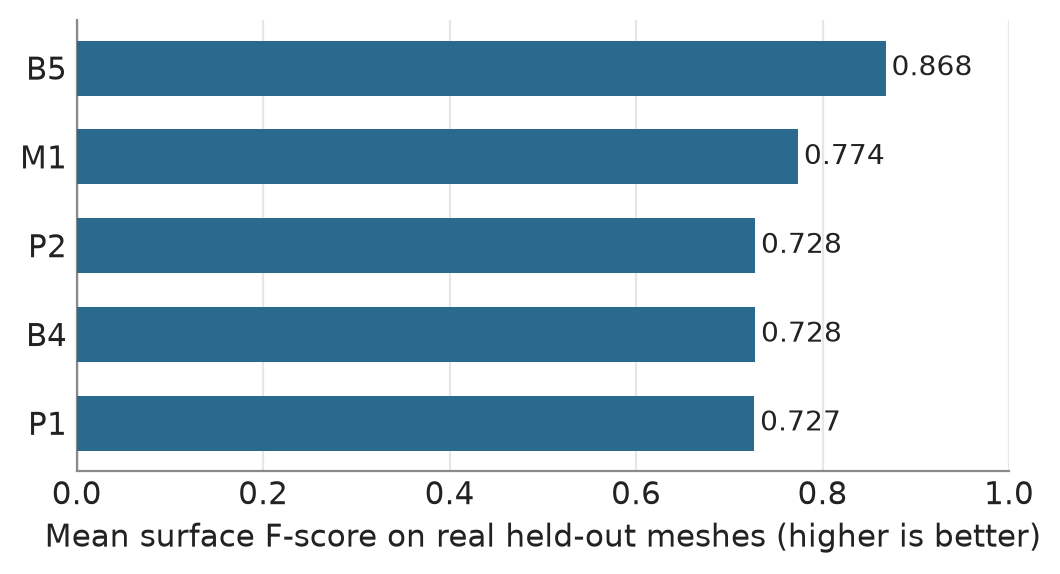
\includegraphics[width=0.72\linewidth]{pics/real_fscore.png}
\caption{Mean surface F-score on the real held-out corpus. The normal-anisotropic
baseline (B5) is best; the weighted regular alpha (M1) improves the density baseline
(B4) but no local-metric candidate (P1, P2, M1) reaches B5.}
\label{fig:fscore}
\end{figure}

\begin{figure}[t]\centering
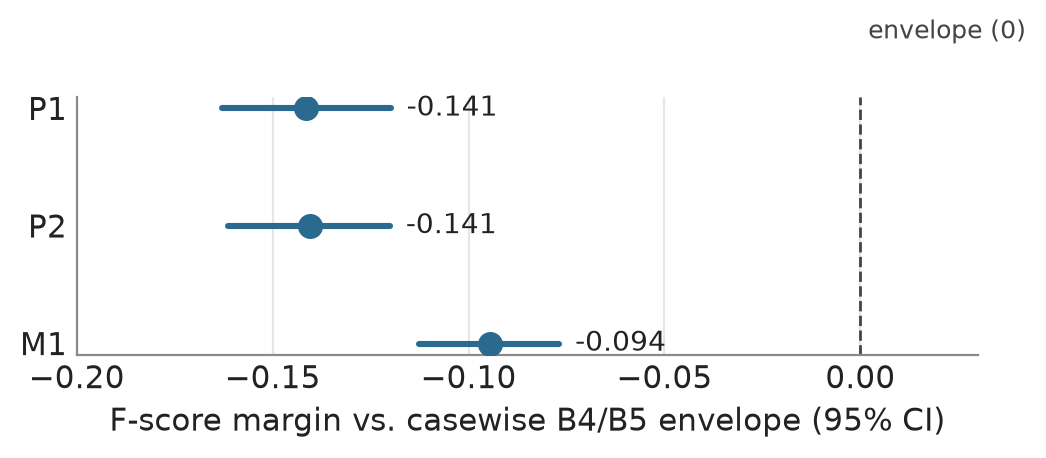
\includegraphics[width=0.72\linewidth]{pics/real_margin.png}
\caption{F-score margin of each candidate against the casewise B4/B5 envelope, with
95\% bootstrap confidence intervals. Every interval is below the zero envelope, so no
candidate clears the held-out gate.}
\label{fig:margin}
\end{figure}

\begin{table}[t]\centering
\caption{Real held-out corpus (40 cases): mean performance and margin against the
casewise baseline envelope $\max(\mathrm{B4},\mathrm{B5})$.}
\label{tab:real}
\begin{tabular}{lccc}
\toprule
Method & Mean F-score & Mean geom.\ loss & F-margin vs.\ $\max(\mathrm{B4},\mathrm{B5})$ \\
\midrule
B4 & 0.728 & 0.094 & --- \\
\textbf{B5} & \textbf{0.868} & \textbf{0.058} & --- \\
P1 & 0.727 & 0.092 & $-0.14$ (0/40 cleared) \\
P2 & 0.728 & 0.092 & $-0.14$ (0/40) \\
M1 & 0.774 & 0.078 & $-0.094$, CI $[-0.11,-0.08]$ (2/40) \\
\bottomrule
\end{tabular}
\end{table}

\subsection{A negative map of false-bridge interventions}
Because false bridges dominate the residual gap, we tried to remove them directly, and
report that every removal-based intervention fails. Per-cell penalties, layered
boundary-owner peeling, connected risk-region removal, a resampling-persistence gate
(discrimination AUC $\approx 0.50$, i.e.\ chance), global multiplier backoff,
reference-free fail-closed routing, and oriented-normal removal, offset and signed
labelling all regress geometry or topology rather than improving them. Two causes
explain the universality of the failure. First, removing a cell from a \emph{fixed}
complex exposes its interior faces as new boundary, so deletion trades a false bridge
for a fresh hole. Second, in the hardest family the inter-surface gap is smaller than
the sample spacing---$41\%$ of kNN edges cross the two ground-truth sheets---so no
\emph{local} method has the information to separate them at all. Only the connectivity
change (M1) helps, and even it does not resolve that under-resolved case, because the
missing information is genuinely absent from local neighbourhoods.

\section{Discussion}
The real held-out evaluation shows, quantitatively and under a deliberately strict
test, that the local SPD metric (P1/P2) provides no reconstruction value beyond the
established normal-anisotropic baseline. The synthetic panel misleads in the opposite
direction: by containing an under-resolved thin-gap pathology it unfairly weakens B5,
so a synthetic-only study could have reported a spurious win for anisotropy. The
divergence between the two settings is itself the lesson---reconstruction claims that
rest on adversarial synthetic panels can invert on realistic meshes, and only a real
held-out test settles the matter.

For AM practice the implication is reassuring and specific. A well-regularised
normal-based metric remains the strong default for scan-to-print reconstruction; the
extra machinery of a directed relation tensor is not worth its cost. What is worth
adopting are the two pieces that survived: the weighted-alpha connectivity change (M1),
which improves the density baseline cheaply and by a mechanism---editing which
simplices exist---that rescoring a fixed complex cannot emulate; and the fail-closed
exact fallback (G4), which lets an exact construction be deployed on the actual
selection path with a guarantee that no failure mode is silently certified as safe, a
property that matters when reconstruction feeds an automated print queue.

Methodologically, the study argues for casewise, multi-endpoint, frozen held-out
evaluation as the default for reconstruction claims. It was exactly this protocol that
demoted P2's small positive mean margin to non-evidence, and it is exactly the kind of
protocol that would prevent the synthetic panel from being over-read.

\section{Limitations and future work}
The evaluation uses a locally assembled corpus rather than a licensed public
leaderboard, and topology endpoints on complex shells are inherently noisy, so the
Betti and nonmanifold figures should be read as directional rather than exact. The
synthetic panel's hardest family is under-resolved by construction and cannot be solved
by any local method, which bounds what any local candidate could have achieved there.

The one avenue our negative results do not foreclose is global: inside/outside labelling
of Delaunay tetrahedra by a minimum-cut over the tetrahedral adjacency graph
\citep{labatut2009}. Unlike every method tested here, such a labelling has, in
principle, access to the global evidence needed to close a thin gap without opening a
hole, precisely because it does not decide cell by cell. Implementing and held-out
testing that labelling---under the same frozen protocol used here---is the natural next
step, and a more promising one than any further local metric.

\section{Conclusion}
We asked whether a PFTF-derived local SPD metric improves anisotropic alpha-complex
surface reconstruction for additive manufacturing, and answered it with a predeclared,
frozen held-out evaluation on synthetic and real data. The answer is negative: on real
held-out meshes a normal-anisotropic baseline is best and no local-metric variant
surpasses it. The study nonetheless yields three reusable results---an improved density
baseline via a weighted regular alpha (M1), a fail-closed exact-construction fallback
with a no-silent-false-safe guarantee (G4), and a documented, mechanistically explained
universal failure of removal-based bridge interventions---and it makes the case for
casewise frozen held-out evaluation as the standard by which such reconstruction claims
should be judged.

% References in Harvard (author-date) style, per RPJ (Emerald).
% Bibliographic details verified against publisher/DOI records (2026-07-25).
\begin{thebibliography}{}
\bibitem[Edelsbrunner(1992)]{edelsbrunner1992}
Edelsbrunner, H. (1992), ``Weighted alpha shapes'', Technical Report UIUCDCS-R-92-1760,
Department of Computer Science, University of Illinois at Urbana-Champaign.

\bibitem[Edelsbrunner and M\"ucke(1994)]{edelsbrunner1994}
Edelsbrunner, H. and M\"ucke, E.P. (1994), ``Three-dimensional alpha shapes'',
\textit{ACM Transactions on Graphics}, Vol.~13 No.~1, pp.~43--72.

\bibitem[Hoppe et al.(1992)]{hoppe1992}
Hoppe, H., DeRose, T., Duchamp, T., McDonald, J. and Stuetzle, W. (1992),
``Surface reconstruction from unorganized points'', \textit{Computer Graphics
(SIGGRAPH)}, Vol.~26 No.~2, pp.~71--78.

\bibitem[Labatut et al.(2009)]{labatut2009}
Labatut, P., Pons, J.-P. and Keriven, R. (2009), ``Robust and efficient surface
reconstruction from range data'', \textit{Computer Graphics Forum}, Vol.~28
No.~8, pp.~2275--2290.

\bibitem[Zhou and Jacobson(2016)]{zhou2016thingi10k}
Zhou, Q. and Jacobson, A. (2016), ``Thingi10K: a dataset of 10{,}000 3D-printing
models'', arXiv:1605.04797.
\end{thebibliography}

\end{document}
